\subproblem
Completar la tabla de de  frecuencias.
\\

En una poblacion de tamaño $n = 500$ familias de una determinada barriada, se ha observado una variable estadística $ X = numero$  de hijos de cada familia que ha presentado $k = 7$ $(0,1,2,3,4,5,6)$ modalidades distintas con la siguiente distribución de frecuencias ($x_{i}$ , $n_{i}$)
	\begin{center}
		\begin{tabular}{ | c | c | c | c | c | c | c | }
	
	
	\hline	
	$x_{i}$ & $n_{i}$ & $N_{i}$ & $f_{i}$ \\ \hline
	0 & 80 & 80  & 0.16 \\
	1 & 110 & 190  & 0.22  \\
	2 & 130 & 320 & 0.26 \\
	3 & 90 & 410  & 0.18 \\ 
	4 & 40 & 450  & 0.08  \\
	5 & 30 & 480 & 0.06 \\
	6 & 20 & 500 & 0.04 \\\hline
	 &  & =500 & =1 \\\hline
	 
\end{tabular}
	\end{center}

Los cálculos realizados para rellenar esta tabla se detallan a continuación: 

		$ N_{0} = n_{0} = 80 $\\ \\
		$ f_{0} = \frac{n_{0}}{n} \rightarrow n = \frac{n_{0}}{f_{0}} =  \frac{80}{16} = 500 $\\ \\
		$ N_{2} = n_{0} + n_{1} + n_{2} = 320 \rightarrow n_{2} = 320 - 190 = 130 $ \\ \\
		$ f_{2} = \frac{n_{2}}{n} = \frac{130}{500} = 0.26$\\ \\
		$ f_{3} = \frac{n_{3}}{n} \rightarrow n_{3} = 500 * 0.18 = 90 $\\ \\
		$ N_{3} =N_{2} + n_{3} = 320 + 90 = 410  $\\ \\
		$ N_{5} =N_{4} + n_{5}  \rightarrow  n_{5}= 500 - n_{0} - n_{1} + n_{2} -n_{3} + n_{4} + n_{6} = 30 $ \\ \\
		$ N_{5} =N_{4} + n_{5} = 450 + 30 = 480 $\\ 
		
		

%\end{table}	
	
\subproblem
Representar la distribución mediante un diagrama de barras y la curva de distribución.

\begin{center}
DIAGRAMA DE BARRAS:
\begin{center}
	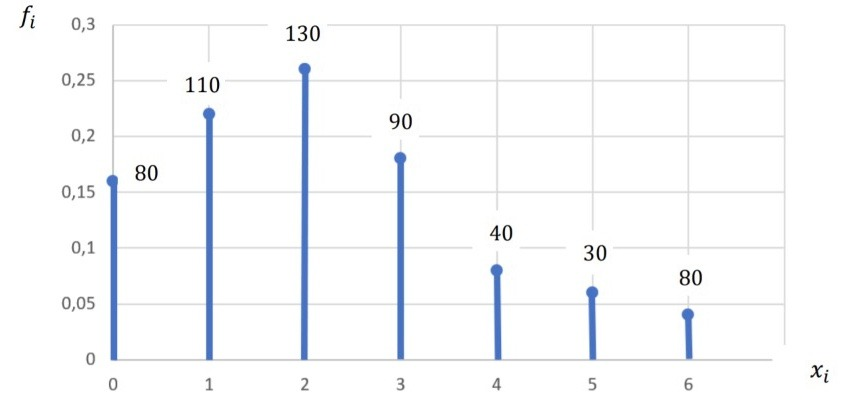
\includegraphics[scale=0.5]{grafica-ej-1.jpeg}

\end{center}
Para el diagrama de barras en el eje X tenemos las modalidades $(x_{i})$ y en el eje Y tenemos las frecuencias relativas acumuladas de cada una de las modalidades $(x_{i})$. \\

\end{center}

\begin{center}

CURVA DE DISTRIBUCIÓN:
\begin{center}
	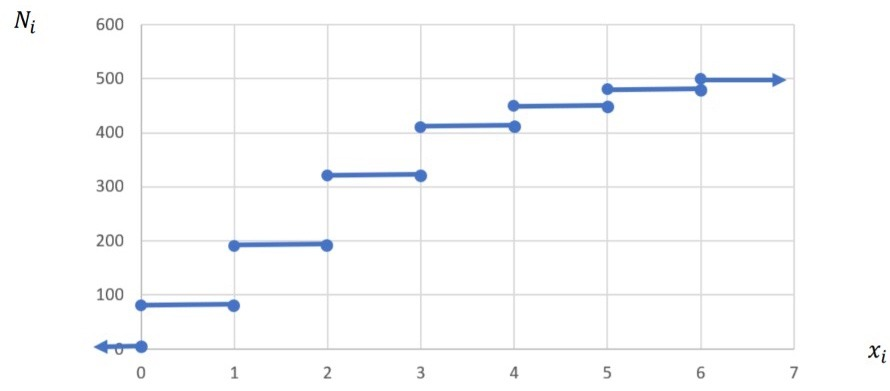
\includegraphics[scale=0.5]{curva-distribucion-ej-1.jpeg}
\end{center}
Para la curva de distribucion en el eje X tenemos las modalidades $(x_{i})$ y en el eje Y tenemos las frecuencias absolutas acumuladas de cada una de las modalidades $(x_{i})$. 
\end{center}
	 \begin{flushleft}
\subproblem
Promediar los valores de la variable mediante diferentes medidas. Interpretarlas.
\end{flushleft}
-MEDIA: en este calcularemos la única que tenga sentido. En este caso es la media aritmética: 
\\
\\
$\bar{x} = \frac{1}{n}  \sum   n_{i} * x_{i}$ 
\\
\\
$\bar{x} = \frac{1}{500} * (110 + 260 +270 + 160 + 150 + 120) = 2.14 $ hijos
\\
\\
-MEDIANA: que es el valor que divide a los individuos de la población en dos efectivos iguales, y para ello buscamos el primer valor cuya frecuencia acumulada sea mayor o igual a $\frac{n}{2}$.
\\
\\
$Me = x_{i} : N_{i} > \frac{n}{2}$
\\

$\frac{500}{2} = 250$ 
\\

$N_{3} > 250  \Rightarrow Me = 2 hijos  $
\\
\\
-Moda: es el valor de mayo frecuencia.
\\
\\
$Mo = x_{i} :x_{i} >= n_{j} \forall j=1,..,7  \Rightarrow Mo = 2 hijos$
\\
\\
\textrightarrow La mediana y la media coinciden en este caso.
\\
\\